\documentclass[10pt]{article} 
\usepackage{fontspec}

\usepackage{mdframed}
\usepackage{amsmath}
\usepackage[space]{xeCJK}
\setCJKmainfont{Noto Sans KR}
\usepackage[a4paper, margin=1in]{geometry}
\setlength{\parindent}{10pt}
\usepackage{graphicx}
\usepackage{setspace}
\usepackage[breakable,skins]{tcolorbox}
\usepackage{enumitem}
\usepackage{cancel}
\usepackage{xcolor}
\usepackage{float}
\usepackage{booktabs}
\usepackage{tabularx}
\usepackage{csquotes}
\usepackage{amssymb}
\usepackage{mathrsfs}
\setstretch{1.3}
\setlength{\jot}{6pt}
\title{
  HI-VQE: Handover Iterative Variational Quantum Eigensolver\\
  for Efficient Quantum Chemistry Calculations
}

\author{
  Aidan Pellow-Jarman \and
  Shane McFarthing \and
  Doo Hyung Kang \and
  Pilsun Yoo \and
  Eyuel E. Elala \and
  Rowan Pellow-Jarman \and
  Prataphorn Nakliang \and
  Jaewan Kim \and
  June-Koo Kevin Rhee
}

\date{
  Qunova Computing, Inc.\\
  Daejeon, Republic of Korea\\[1ex]
  March 18, 2025
}


\begin{document}


\maketitle

\section{Introduction}
{\Large $\bullet$ Ground-State Energy}

배터리개발분야, 혹은 신약개발분야, 혹은 반도체분야 등 화학반응을 사용하는 분야에 있어서 분자의 바닥상태 에너지를 계산하는것은 매우 중요한 일중 하나이다. 
\begin{figure}[htbp]
  \centering
  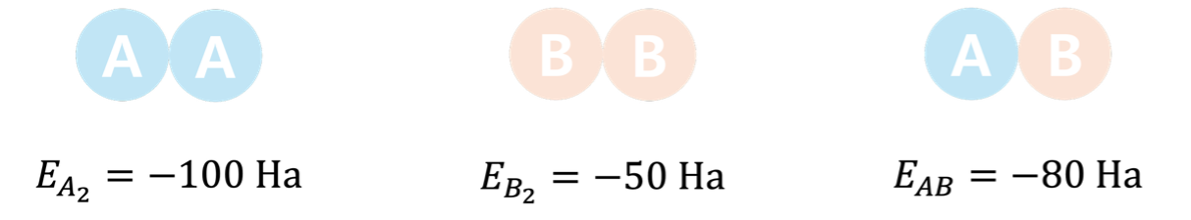
\includegraphics[width=0.8\textwidth]{fig/Eg예시.png}
  \caption{바닥상태 에너지 예시}
  \label{fig:example}
\end{figure}

위와같이 A\(_2\) 분자의 바닥상태 에너지는 -100 Ha, B\(_2\) 분자의 바닥상태 에너지는 -50 Ha, AB 분자의 바닥상태 에너지는 -80 Ha 정도인 상황을 보자. 여기서 Ha는 아래와같은 에너지단위이다:

\[
1~Ha = m_e R_y^2 \quad \textit{where} \quad m_e: \text{mass of Electron}, \quad R_b: \text{Bohr Radius}
\]

이런 상황에서, 어떤 진공 박스에 A\(_2\) 분자 1개와 B\(_2\) 분자 1개를 넣었다고 해보자. 
여기서, 우리는 일반적으로 시스템은 더 안정화된다는 경향이 있다는 물리적인 직관을 갖고 있다. 
즉, 어떤 시스템이 있으면, 그 에너지는 더욱 낮아지려고할것이다.

그런데 여기서, A\(_2\), B\(_2\) 가 각각 단분자로 존재한다고 하면 그 시스템이 갖는 에너지는 -150 Ha 일것이다. 
그런데, A와 B가 만나서 AB를 만들면, 하나의 AB 분자가 갖는 에너지는 -80 Ha 가 된다. 
따라서  그 시스템이 갖는 에너지는 -160 Ha 일것이고, 에너지가 더 낮아지므로 이렇게 되는것이 더 안정적인 상태이다.
즉, 박스안에 두 A\(_2\), B\(_2\) 분자를 넣었을때 아마 두 분자는 결합하여 2개의 AB 분자가 될것이다. 

\[
A_2 + B_2 \rightarrow 2AB
\]
더 일반적으로 제약분야와같은 상황을 생각할때, 어떤 약을 투여했을때, 그 약이 어떤 부위에 작용할것인가, 또 붙어서 어떤 반응을 작용할것인가 등의 현상이 가장 중요한 고민사항 일것이다.
이는 물리학자의 시선에서 에너지의 관점으로 바라보면, 이러한 작용들이 결국 전체 계의 에너지가 낮아지는 방향으로 진행될것임을 알 수 있고,
따라서 바닥상태 에너지의 계산을 통해 이러한 작용들을 이해할 수 있을것이라는 기대를 가질 수 있다.

이러한 논리는 분명 엄밀하지 않다. 단순히 바닥상태 에너지만을 이용해서 화학 반응을 계산할 수 있는것은 아니다. 
하지만 그럼에도 바닥상태 에너지가 그 반응에 있어 중요한 물리량 중 하나라는것을 직관적으로는 이해할 수 있을것이다. 
더 엄밀하게는, Gibbs 자유에너지를 계산해야하는데, 이 계산에는 바닥상태에너지가 필요하다. 
또한 특히 배터리 분야에서 생각한다면, 최근의 배터리 분야의 최대목적은 배터리의 소형화이다. 
이는 1) 산업적인 측면에서 배터리의 물리적인 크기를 줄이는것은 경제적인 이점이 있고, 
2) 리튬, 혹은 배터리에 사용되는 코발트 등 희토류 원소들은 그 자체로 최근 전쟁의 원인이 될정도로 지구상에 매우 한정적인 재료이다. 
그러한 재료를 덜 사용하고 같은 성능을 낸다 라는것은 환경적인 이유에서도 큰 이점이 될 수 있다. 
이러한 맥락에서 중요한것이 바로 “에너지 밀도” 이다. 즉, 부피당, 혹은 리튬이온 하나당 얼만큼의 에너지를 저장할 수 있는가가 매우 중요한 상황인데,
 이 에너지 밀도의 계산에서 화합물들의 바닥상태에너지의 계산이 필요하다.


\section*{HIVQE의 등장배경}


지금까지의 이야기를 통해 바닥상태 에너지 계산은 현대산업에 있어서 매우 중요한 계산이라는것을 이해할 수 있었다. 그럼 그 바닥상태 에너지는 어떻게 계산한다는가? 중요한 이야기일것이어서 쉽게 쉬웠으면 좋게 명확하게 이야기하지도 않았을것이다.



\begin{enumerate}[label=\arabic*)]
\item {\Large \textbf{Analytic Solution}}

결국 바닥상태 에너지라는것은 그 시스템이 갖는 가장 낮은 에너지일것이고, 이는 분자이므로 이문제의 물리는 양자역학으로밖에 해결할수 없었겠으며, 
이러한 시스템의 에너지를 계산하는 문제는 단순하게 아래와같이 슈뢰딩거 방정식을 해결하여 얻을 수 있다. 

\[
\hat{H}|\Psi\rangle = E|\Psi\rangle \longrightarrow
\left\{
\begin{aligned}
|\Psi\rangle &= \sum_n a_n |\psi_n \rangle \\
E_n &= \langle \psi_n | H | \psi_n \rangle
\end{aligned}
\right.
\]
근데 이게 쉽냐 하면 절대로 쉽지않다.  
일단 헤밀토니안에 따라 달라지겠지만, 물리학에서의 에너지는 보통 어떤 위치나 운동량과 같은 Cannonical 한 물리량의 제곱에 해당하는 항으로 주어지게 되고, 
보통 그렇기 때문에 슈뢰딩거방정식은 비선형 미분방정식이 된다. 
분자도 아니고, 원자를 보자. 원자중에서 가장 간단한 원자는 수소원자일것이고 
수소원자에서 위에서 파동함수와 에너지를 계산해보면, 아래와같다.
\begin{align*}
\psi_{nlm}(r, \theta, \phi) &= R_{nl}(r) Y_l^m(\theta, \phi) \\
R_{nl}(r) &= N_{nl} \left(\frac{2r}{na_0}\right)^l e^{-\frac{r}{na_0}} L_{n-l-1}^{2l+1}\left(\frac{2r}{na_0}\right) \\
Y_l^m(\theta, \phi) &= N_{lm} P_l^m(\cos \theta) e^{im\phi} \\
E_n &= -\left(\frac{m_e e^4}{8 \varepsilon_0^2 h^2}\right) \frac{1}{n^2}
\end{align*}
위의 표현에서 n=1 일때를 찾아본다면, 수소원자의 바닥상태와 바닥상태 에너지를 얻을 수 있을것이다. 
수리물리학을 잘 공부했다면, 이렇게 표현되는것 자체는 복잡하긴 해도 받아들일 수 있을것이다. 
하지만 말하고자 하는 내용은 아주 복잡하다는것이다. 
실제로, 이렇게 슈뢰딩거 방정식을 풀어 해를 얻는것이 가능한것은, 수소, 혹은 수소와같이 최외곽 전자가 하나인 원자뿐이다. 
거기다 이건 단순히 “원자”의 이야기이다. 우리가 결국 풀고자 하는 문제는 분자에 관한 문제이다. 분자에 대해서도 마찬가지로 이러한 해석적인 방법으로는 해결할 수 없다. 
그래서 이러한 문제를 해결하기 위해, 물리학자들은 많은 방식들을 시도하였고, 그중의 한가지 방식을 소개하겠다. 그 방식이 이후 VQE에도 사용될것이다. 
\end{enumerate}

\begin{enumerate}[label=2)]
\item {\Large \textbf{Variational Method}}
우리가 마주하고 있는 문제는 아래와같은 슈뢰딩거방정식이다.

\[
\hat{H}|\Psi\rangle = E|\Psi\rangle
\]

그런데 여기서 $|\Psi\rangle$를 구하는 것이 어려워 $E$를 구할 수 없었다. 
그래서 이렇게 시도를 해보는것이다. $|\Psi\rangle$를 우리가 어떤 파라미터를 포함한 형태로 임의로 구성하는것이다. 
이때는, 풀고자하는 시스템의 파동함수와 유사한 파동함수를 택할수도 있고,
혹은 임의의 Hilbert 공간의 함수를 표현할 수 있는 complete한 (현실적으로는 Complete 할것이라고 기대되는) 함수를 이용해서 표현할 수 있다.

어떻게든 함수를 파라미터를 포함한 형태로 표현하게되면,
\[
E(\theta) = \langle \Psi(\theta) | H | \Psi(\theta) \rangle
\]

에너지를 계산할 수 있고, 그 에너지는 파라미터에 대해 Explicit 하게 표현이 된다. 
그렇게되면 그 파라미터에 대해서 최적화 하여 우리가 구성한 함수 내에서 표현될 수 있는 가장 낮은 에너지를 계산할 수 있다. 
이제 여기서 한가지 논리를 생각해볼 수 있다.

\begin{enumerate}[label=*]
\item  \textbf{그 에너지가 과연 합리적인가? 그렇게 계산하는게 무슨 의미인가?}

이에 대한 논리를 주는 것이 Variational Principle 이다.

\begin{tcolorbox}[enhanced, breakable, colback=gray!10, colframe=black, title=Definition: Variation Principle]

\[
\langle \Psi | \hat{H} | \Psi \rangle \geq E_{\text{ground}}
\]

즉, 어떻게 상태를 구성하여 기대값을 측정하더라도 그 기대값의 계산결과는 항상 $E_{\text{ground}}$보다 크다.

\end{tcolorbox}

\begin{mdframed}
\textit{proof.} \\
Observable인 $\hat{H}$ 연산자는 Hermitian 이다. Hermitian 연산자는 언제나 orthonormal한 basis를 가진다. 즉, 아래의 고유치 방정식을 만들 수 있고,
\[
\hat{H} |e_i \rangle = E_i |e_i \rangle, \quad \langle e_i | e_j \rangle = \delta_{ij}
\]
그 Hilbert space에 존재하는 임의의 상태를 basis를 이용하여 아래와같이 표현할 수 있다.
\[
|\Psi_{\text{arbitrary}}\rangle = \sum_i c_i |e_i\rangle \tag{1}
\]

그리고 각 고유상태는 정규화 되어있다고 하자.
\[
\langle \Psi | \Psi \rangle = 1
\]


위에서 정의한 임의의 상태를 이용해 해밀토니안의 기대값, 즉 에너지를 계산해보면 아래와같다.

\begin{align*}
E_\Psi &= \langle \Psi | \hat{H} | \Psi \rangle \\
&= \left\langle \sum_i c_i e_i \left| \hat{H} \right| \sum_j c_j e_j \right\rangle \\
&= \sum_{i} \sum_{j} c_i^* c_j \langle e_i | \hat{H} | e_j \rangle \\
&= \sum_{i} \sum_{j} c_i^* c_j \langle e_i | E_j e_j \rangle \\
&= \sum_{i} \sum_{j} c_i^* c_j E_j \langle e_i | e_j \rangle \\
&= \sum_{i} c_i^* c_i E_i \\
&= \sum_{i} |c_i|^2 E_i \tag{2}
\end{align*}

즉,
\[
E_\Psi = \sum_{i} |c_i|^2 E_i
\]

임의의 상태는 고유상태에 대한 선형결합으로 표현될것이다. 그리고 그 상태의 에너지를 계산해보게되면, 각 고유상태에 대응되는 에너지와 그 선형계수의 제곱의 가중치합을 갖고 얻을 수 있다.

편의상 인덱스를 아래와같이 주자.
\[
E_0 (= E_{\text{ground}}) < E_1 < E_2 < \cdots
\]

각 에너지는 각 고유상태에 대응되는 에너지이므로, 그럼 바닥상태는 자연스럽게 아래와같이 표현할 수 있을것이다.
\[
|\Psi_{\text{ground}}\rangle = c_0 | e_0 \rangle = 1 \cdot | e_0 \rangle
\]

이 내용을 가지고 아래의 식을 쳐다보자.
\[
|\Psi_{\text{arbitrary}}\rangle = \sum_i c_i | e_i \rangle
\]
\[
E_\Psi = \sum_{i} |c_i|^2 E_i
\]

바닥상태인 상태는 "유일(unique)"하게 아래의 조건을 만족한다.
\[
c_0=1, \quad c_1=0, \quad c_2=0, \quad \cdots, \quad c_i=0 \; (i \neq 0)
\]

0이 아닌 인덱스에 대한 에너지가 아래와같이 약속했으므로,
\[
E_0 (= E_{\text{ground}}) < E_1 < E_2 < \cdots
\]

따라서 그 외의 조건에서 일반적인 상태에 대한 에너지는 바닥상태에너지보다 크게된다.
\[
E_\Psi = \sum_i |c_i|^2 E_i \ge E_0
\]
\end{mdframed}
즉, Variational Method를 통해 계산된 에너지는 바닥상태 에너지를 Lower Bound로 가지게 된다. 
즉, Variational Method를 통해 계산된 에너지를 계속해서 에너지가 낮아지는 방향으로 최적화를 진행하게 되면, 결국 다다르게 되는 에너지는 특정 basis 에서 헤밀토니안이 가질 수 있는 Ground-state energy가 되게 된다. 

\end{enumerate}

이러한 Variational Method에대한 간단한 예제가 있고 이것에 대해 이해해보자. 

\begin{mdframed}
\underline{\textbf{Variational Method 예제 (Quantum Harmonic Oscillator)}}

Quantum Harmonic Oscillator 시스템에서의 헤밀토니안은 아래와같다. 
\[H = -\frac{\hbar^2}{2m}\frac{d^2}{dx^2} + \frac{1}{2}m\omega^2 x^2 \]
사실 이거 풀수 있긴한데, 풀 줄 모른다고 해보자. 그럼 우리의 논리대로라면, 그 모르는 파동함수를 우리가 잘 아는 어떤 함수의 꼴로 구성해야할것이다. 
이 "잘 아는" 함수로 Gaussian 을 사용해보자. 
\[
\psi(x) = Ae^{-bx^2}
\]
이때 A 는 정규화 조건을 통해 구할 수 있다. 
\begin{align*}
1 &= |\psi(x)|^2  \\
&= |A|^2 \int_{-\infty}^{\infty} Ae^{-2bx^2} \, dx \\
&= |A|^2 \sqrt{\frac{\pi}{2b}}
\end{align*}
\[
\longrightarrow A = \left(\frac{2b}{\pi}\right)^{\frac{1}{4}}
\]
그럼이제 파동함수는 아래와같이 쓸 수 있다. 
\[
\psi(b,x) = \left(\frac{2b}{\pi}\right)^{\frac{1}{4}}e^{-bx^2}
\]
그리고 이 상태에서 앞선 논리대로 임의의 파동함수(양자상태)에 대해서 기댓값을 측정하여, 
에너지를 파라미터 b에 대해 Explicit 하게 표현해보자.
\begin{align*}
E(b) &= \langle H \rangle \\
&= \langle T \rangle + \langle V \rangle \\
&=\langle \psi|T|\psi \rangle + \langle \psi|V|\psi \rangle \\
&=\frac{\hbar^2 b}{2m} + \frac{m\omega^2}{8b}
\end{align*}


이제 저 파동함수를 통해 기술되는 에너지의 최솟값을 얻기위해 b에 대해 미분하자(최적화 과정). 
\begin{align*}
\frac{d}{db} E &= \frac{\hbar^2}{2m} - \frac{m \omega^2}{8b^2} \\
&\Longrightarrow b_0 = \frac{m\omega}{2\hbar}
\end{align*}

따라서 최적화된 파라미터를 에너지에 대입하면, 우리의 시험 파동함수(Ansatz)를 통해 기술되는 에너지의 최솟값을 계산할 수 있다. 
\[
E(b_0) = \frac{1}{2}\hbar\omega
\]
\[
cf, \quad E_{Analytic} = \frac{1}{2}\hbar\omega
\]
\end{mdframed}
이경우는 우리가 파동함수의 형태를 "우연히" 잘 잡아서 Exact 한 해와 같은 형태로 기술된다. 
이때, 저 함수의 형태를 어떤식으로 잡던지 저 값보다 작은 값은 얻을 수 없다(due to Variational Principle)
다른 시스템에서도 이처럼, 파동함수를 잘 기술하면 바닥상태 에너지에 가까운 에너지를 얻을 수있다. 
이런식으로 에너지를 계산하는것이 Variational Method 이다. 

자 그런데, 일반적으로, 파동함수을 단순하게 Gaussian 하나만으로 만들지는 않을것이다. 
예를들어 N개의 함수의 선형결합이라고 해보자. 
그러면, 이방식으로 문제를 진행하려면 결국 \(\langle H \rangle \\\)를 계산해야한다. 그리고 이때 총 적분해야할 항은 \(N^2\)개가 되게된다. 
우리가 결국 풀고자하는 분자의 시스템에서의 헤밀토니안은 쿨롱퍼텐셜항에 의해 \(\frac{1}{r}\)항이 생기게되고, 당연히 적분구간은 \(0~\infty\) 이다. 
이때 저 0이라는 구간때문에, 에너지가 발산해버리게되어서, 일반적으로는 적분이 안되고 수학적인 트릭들을 사용해야하는데, 이때 이러한 적분이 코스트가 크다. 
또, 일반적으로 저 N개를 택할때 몇억, 몇십억개의 basis를 사용하게되어 실질적으로 계산이 어렵다. 
따라서 이를 해결하기 위해 저 적분계산을 좀 쉽게 할수있는 방법이 없을까? 에대한 맥락에서 저 적분계산을 양자컴퓨터에서 돌려보자 라는 아이디어를 적용한 방식이 바로 VQE(Variational Quantum Eigensolver)이다. 

\vspace{\baselineskip}
\end{enumerate}

\begin{enumerate}[label=3)]
\item {\Large \textbf{VQE(Variational Quantum Eigensolver)}}

이 섹션만 해도 하고싶은, 해야할 이야기가 산더미처럼 있지만, 이 노트에서 정리하고싶은 내용이 VQE는 아니기때문에 여기는 간단한 스토리정도만 요약해보겠다.([1] 참고.)
2) Variational Method 에서 3)VQE 로 넘어가는 과정에서, 그럼 우리가 해야할것은 결국 \(\langle \psi|H|\psi \rangle\)를 파라미터화된 형태로 구성하고, 양자컴퓨터에서 계산하는 방법을 찾는것이다. 
이과정을 크게 파트별로 \(\mathrm{i}\)) hamiltonian의 구성, \(\mathrm{ii}\))Ansatz의 구성, \(\mathrm{iii}\)) \(\langle \psi|H|\psi \rangle\)의 계산 의 순서로 이해해보자. 
\begin{enumerate}[label=\(\mathrm{i}\))]
\item {\(H\)\,\textbf{(hamiltonian)}}

\begin{figure}[htbp]
  \centering
  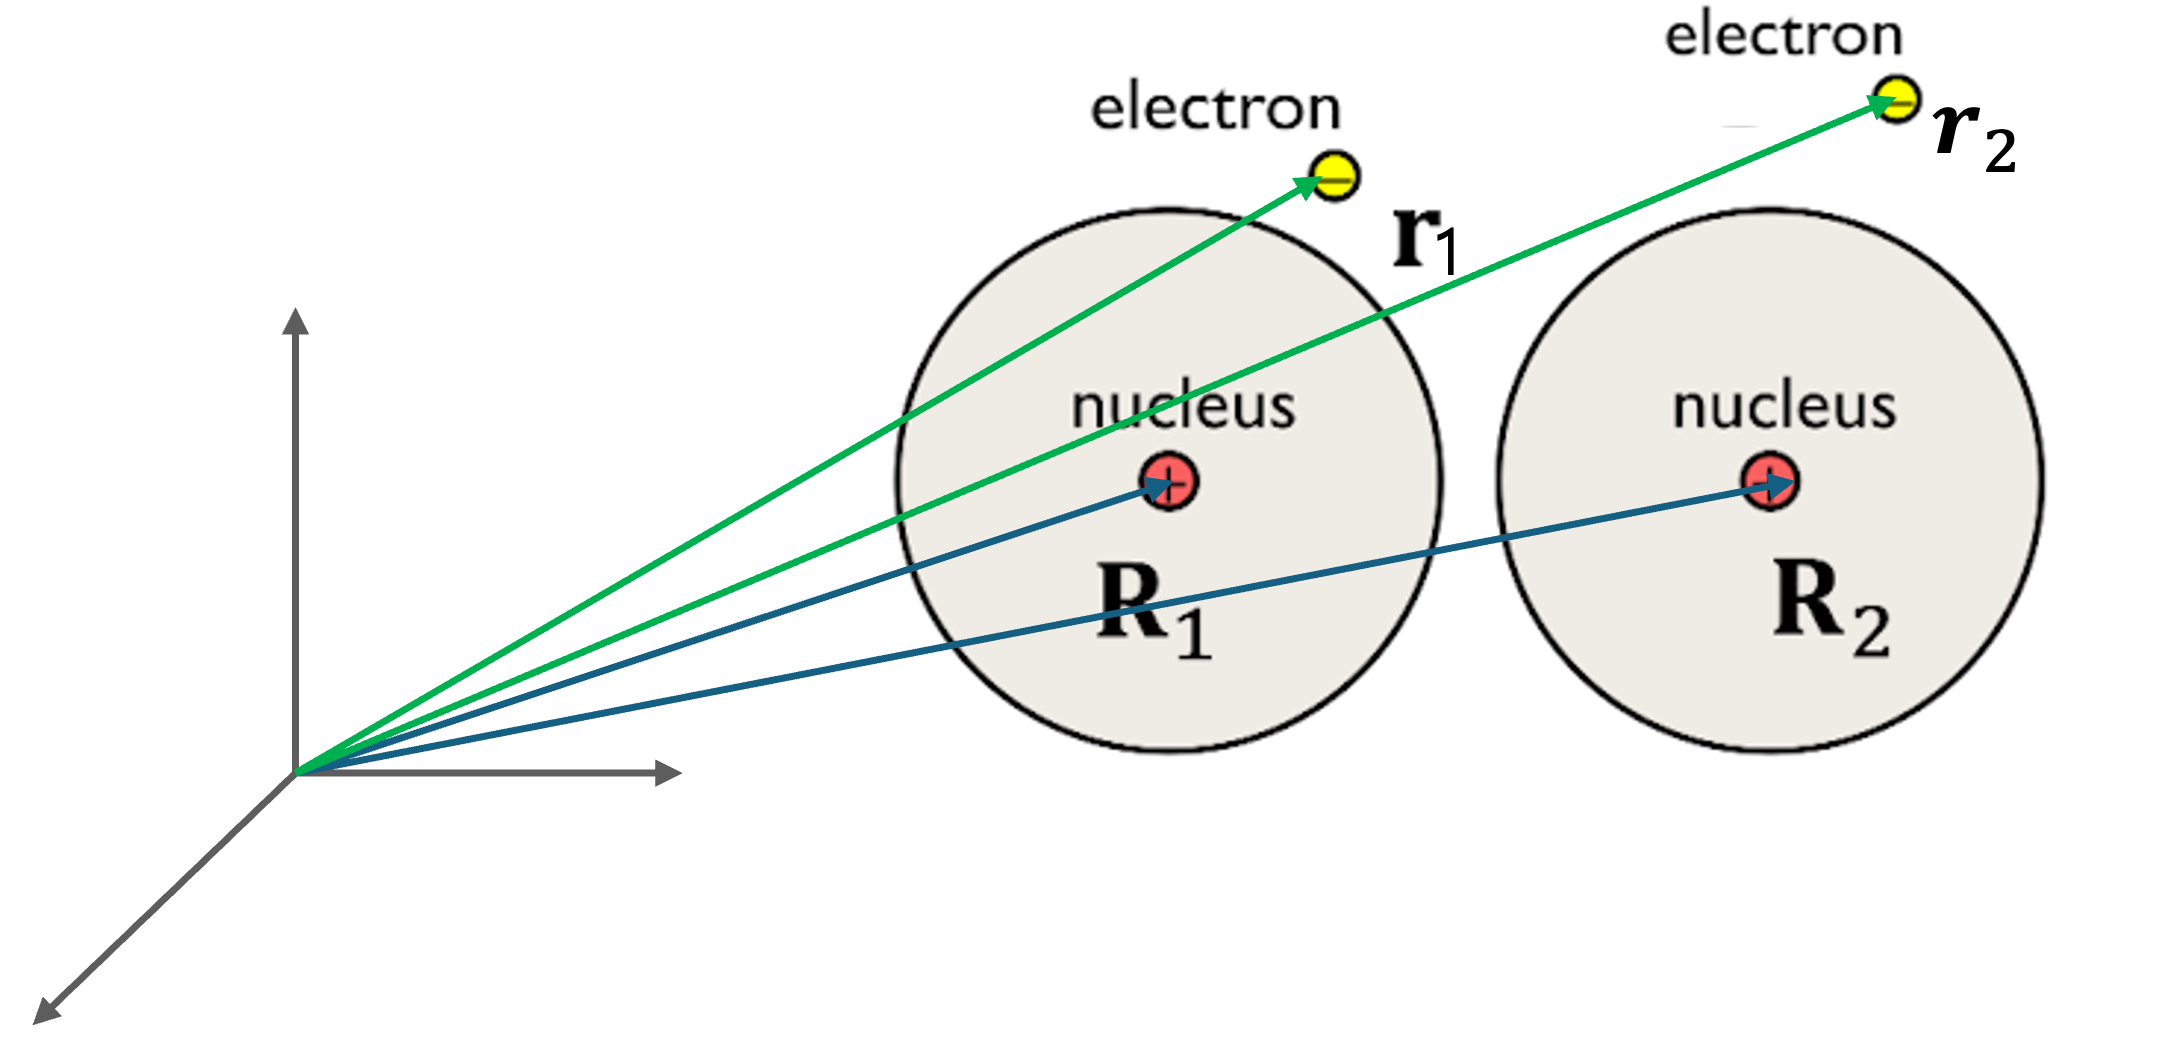
\includegraphics[width=0.5\textwidth]{fig/원자좌표.png}
  \caption{원자에서의 좌표 모식도}
  \label{fig:example2}
\end{figure}

그림 2와 같은 시스템을 보자. 여기서 고려 할 수 있는 헤밀토니안의 항은 아래와같다. 
\[
\hat{H}_{\text{elec}} = \hat{K}_{\text{atom}} + \hat{K}_{\text{elec}} 
+ \hat{V}_{\text{elec-nuclei}} + \hat{V}_{\text{elec-elec}} + \hat{V}_{\text{nuclei-nuclei}}
\]
그리고 각 항을 표현하면 아래와같이 표현된다. 
\[
\hat{H}_{\text{elec}} = - \sum_I \frac{\hbar^2}{2 M_I} \nabla_I^2
- \sum_i \frac{\hbar^2}{2 m_e} \nabla_i^2
- \frac{1}{2} \sum_{I,i} \frac{e^2}{4 \pi \epsilon_0} \frac{Z_I}{|\mathbf{r}_i - \mathbf{R}_I|}
- \frac{1}{2} \sum_{i \ne j} \frac{e^2}{4 \pi \epsilon_0} \frac{1}{|\mathbf{r}_i - \mathbf{r}_j|}
+ \frac{1}{2} \sum_{I,J} \frac{e^2}{4 \pi \epsilon_0} \frac{Z_I Z_J}{|\mathbf{R}_I - \mathbf{R}_J|}
\]

우선 여기에 \underline{a) Born-Oppenheimer 근사를 적용한다.} 
\begin{tcolorbox}[enhanced, breakable, colback=gray!10, colframe=black, title=Definition: Born-oppenheimer Approximation]


\begin{minipage}[t]{0.48\textwidth}
  \vspace*{0pt} % 그림을 minipage 맨 위로 올림
  \centering
  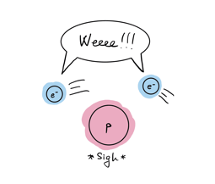
\includegraphics[width=\linewidth]{fig/BOapprox.png}
  \vspace{6pt}
  \textbf{Figure:} BO approximation diagram
\end{minipage}
\hfill
\begin{minipage}[t]{0.48\textwidth}
  \vspace*{10pt} % 텍스트도 minipage 맨 위로 정렬
  핵의 움직임이 전자에 비해 충분히 느려 핵의 움직임을 무시할 수 있다. 

\vspace*{8pt}

\(\rightarrow \mathbf{R}_I\) : Constant

\vspace{\baselineskip}

\(\rightarrow \sum_{i \ne j} \frac{e^2}{4 \pi \epsilon_0} \frac{1}{|\mathbf{r}_i - \mathbf{r}_j|} = 0\) 

\vspace{\baselineskip}

\(\rightarrow \sum_{I,J} \frac{e^2}{4 \pi \epsilon_0} \frac{Z_I Z_J}{|\mathbf{R}_I - \mathbf{R}_J|}\) : Constant

\vspace*{5pt}

(고유치 문제에서 상수는 고유벡터에 영향을 주지 않으므로 무시 하고 나중에 고려)

\end{minipage}

\end{tcolorbox}

이러한 근사방식은 분자계산에서 매우 합리적으로 받아들여지고 있고 이러한 근사를 적용하게되면 헤밀토니안은 아래와 같이 적을 수 있다. 
\[
\hat{H} = -\sum_i \frac{\hbar^2}{2 m_e}\nabla_{r_i}^2 -  \sum_I \sum_i \frac{e^2}{4\pi \epsilon_0}\frac{Z_I}{|\mathbf{r}_i-\mathbf{R}_I|}
+ \sum_i \sum_{j>i} \frac{e^2}{4\pi \epsilon_0} \frac{1}{|\mathbf{r}_i - \mathbf{r}_j|} + \cancelto{neglect! \, (in \,now)}{Const.}
\]

이 표현을 무차원변수로 만들어 주기 위해 \underline{b) atomic units 으로 표현하자.} 
\[Let.\quad r=\lambda r', \quad R=\lambda R'\]
여기서\(\lambda\) 를 Bohr Radius 로 잡게되면,
\[\lambda=\frac{4\pi\epsilon_0\hbar^2}{m_ee^2} (=\text{Bohr Radius})\]
헤밀토니안을 아래와같이 정리할 수있다. 
\begin{align*}
\hat{H} &= -\sum_i \frac{\hbar^2}{2 m_e{\color{red} {\lambda^2}}}\nabla_{r_i'}^2 -  \sum_I \sum_i \frac{e^2}{4\pi \epsilon_0{\color{red} {\lambda}}}\frac{Z_I}{|\mathbf{r'}_i-\mathbf{R'}_I|}
+ \sum_i \sum_{j>i} \frac{e^2}{4\pi \epsilon_0{\color{red} {\lambda}}} \frac{1}{|\mathbf{r'}_i - \mathbf{r'}_j|} \\
&=\left(\frac{m_ee^4}{16\pi^2\epsilon^2\hbar^2}\right)\left[-\sum_i \frac{1}{2}\nabla_{r_i}^2 -  \sum_I \sum_i \frac{Z_I}{|\mathbf{r}_i-\mathbf{R}_I|}
+ \sum_i \sum_{j>i} \frac{1}{|\mathbf{r}_i - \mathbf{r}_j|}\right]
\end{align*}
이러한 헤밀토니안으로 구성되는 슈뢰딩거방정식을 생각해보면 아래와같고. 
\begin{align*}
\hat{H}\vert\psi\rangle &= \left(\frac{m_ee^4}{16\pi^2\epsilon^2\hbar^2}\right)\left[-\sum_i \frac{1}{2}\nabla_{r_i}^2 -  \sum_I \sum_i \frac{Z_I}{|\mathbf{r}_i-\mathbf{R}_I|}
+ \sum_i \sum_{j>i} \frac{1}{|\mathbf{r}_i - \mathbf{r}_j|}\right]\vert\psi\rangle\\
&=E\vert\psi\rangle
\end{align*}
따라서 상수항을 에너지항으로 넘기면 아래와같이 정리할 수있다. 
\[
\left[-\sum_i \frac{1}{2}\nabla_{r_i}^2 -  \sum_I \sum_i \frac{Z_I}{|\mathbf{r}_i-\mathbf{R}_I|}
+ \sum_i \sum_{j>i} \frac{1}{|\mathbf{r}_i - \mathbf{r}_j|}\right]\vert\psi\rangle = {\color{blue}\left(\frac{16\pi^2\epsilon^2\hbar^2}{m_ee^4}\right)E} \vert\psi\rangle
\]

여기서 우변의 저 새로운 에너지를  단위 (or Atomic Unit) 에너지 라고 한다. 
\[
\left(\frac{16\pi^2\epsilon^2\hbar^2}{m_ee^4}\right)E[J] = E[]
\]


\(\left(\frac{16\pi^2\epsilon^2\hbar^2}{m_ee^4}\right)\) 는 계산해보면 \(1/E\)의 차원을 가지므로 우변 또한 무차원 변수로 표현되게 된다. 

여기에 우리가 풀 시스템이 전자(Fermion)로 구성되어있고, 그 시스템이 오비탈에 의해 양자화 되어있다는 사실에 착안하여, 생성/소멸 연산자를 정의하여 아래와같이 Second Quantized 된 형태로 표현할 수있다. 
\[
\hat{H} = \sum_{p,q} h_{pq} \hat{a}_p^\dagger \hat{a}_q
+ \frac{1}{2} \sum_{p,q,r,s} h_{pqrs} \hat{a}_p^\dagger \hat{a}_q^\dagger \hat{a}_r \hat{a}_s
\]

그리고 여기에 각 생성/소멸 연산자를 파울리 연산자로표현하는 Mapping(Jordan-Wigner, parity,...)을 사용하여 아래와같이 파울리 연산자(정확히는 파울리 스트링)의 형태로 표현할 수 있다. 
\[
\hat{H} = \sum_{a} \omega_a P_a, \quad \text{where} \quad
P_a = \hat{p}_0 \otimes \hat{p}_1 \otimes \cdots \otimes \hat{p}_N, \quad
\hat{p}_i \in \{I, X, Y, Z\}
\]

긴 과정을 거쳤지만, 결국 우리가 한것은 r이라는 변수로 표현되었던 헤밀토니안을, 파울리 연산자를 통해 표현하였고, 이 헤밀토니안이 이후 계산에서 사용될것이다. 

\end{enumerate}

\begin{enumerate}[label=\(\mathrm{ii}\))]
\item {Ansatz}


결국 여기서 해야할것은, 파라미터를 통해 표현된 양자상태 특히 VQE에서는 양자회로를 만들어야한다. 
그러기위해 생각할수 있는 두가지의 방법이 있을것이다. 

첫째는, 정말로 양자컴퓨터에서 임의의 양자상태를 만드는것이다. 따라서 이는 Hardware-Efficient 한 방법일것이다. 

\begin{figure}[H]
  \centering
  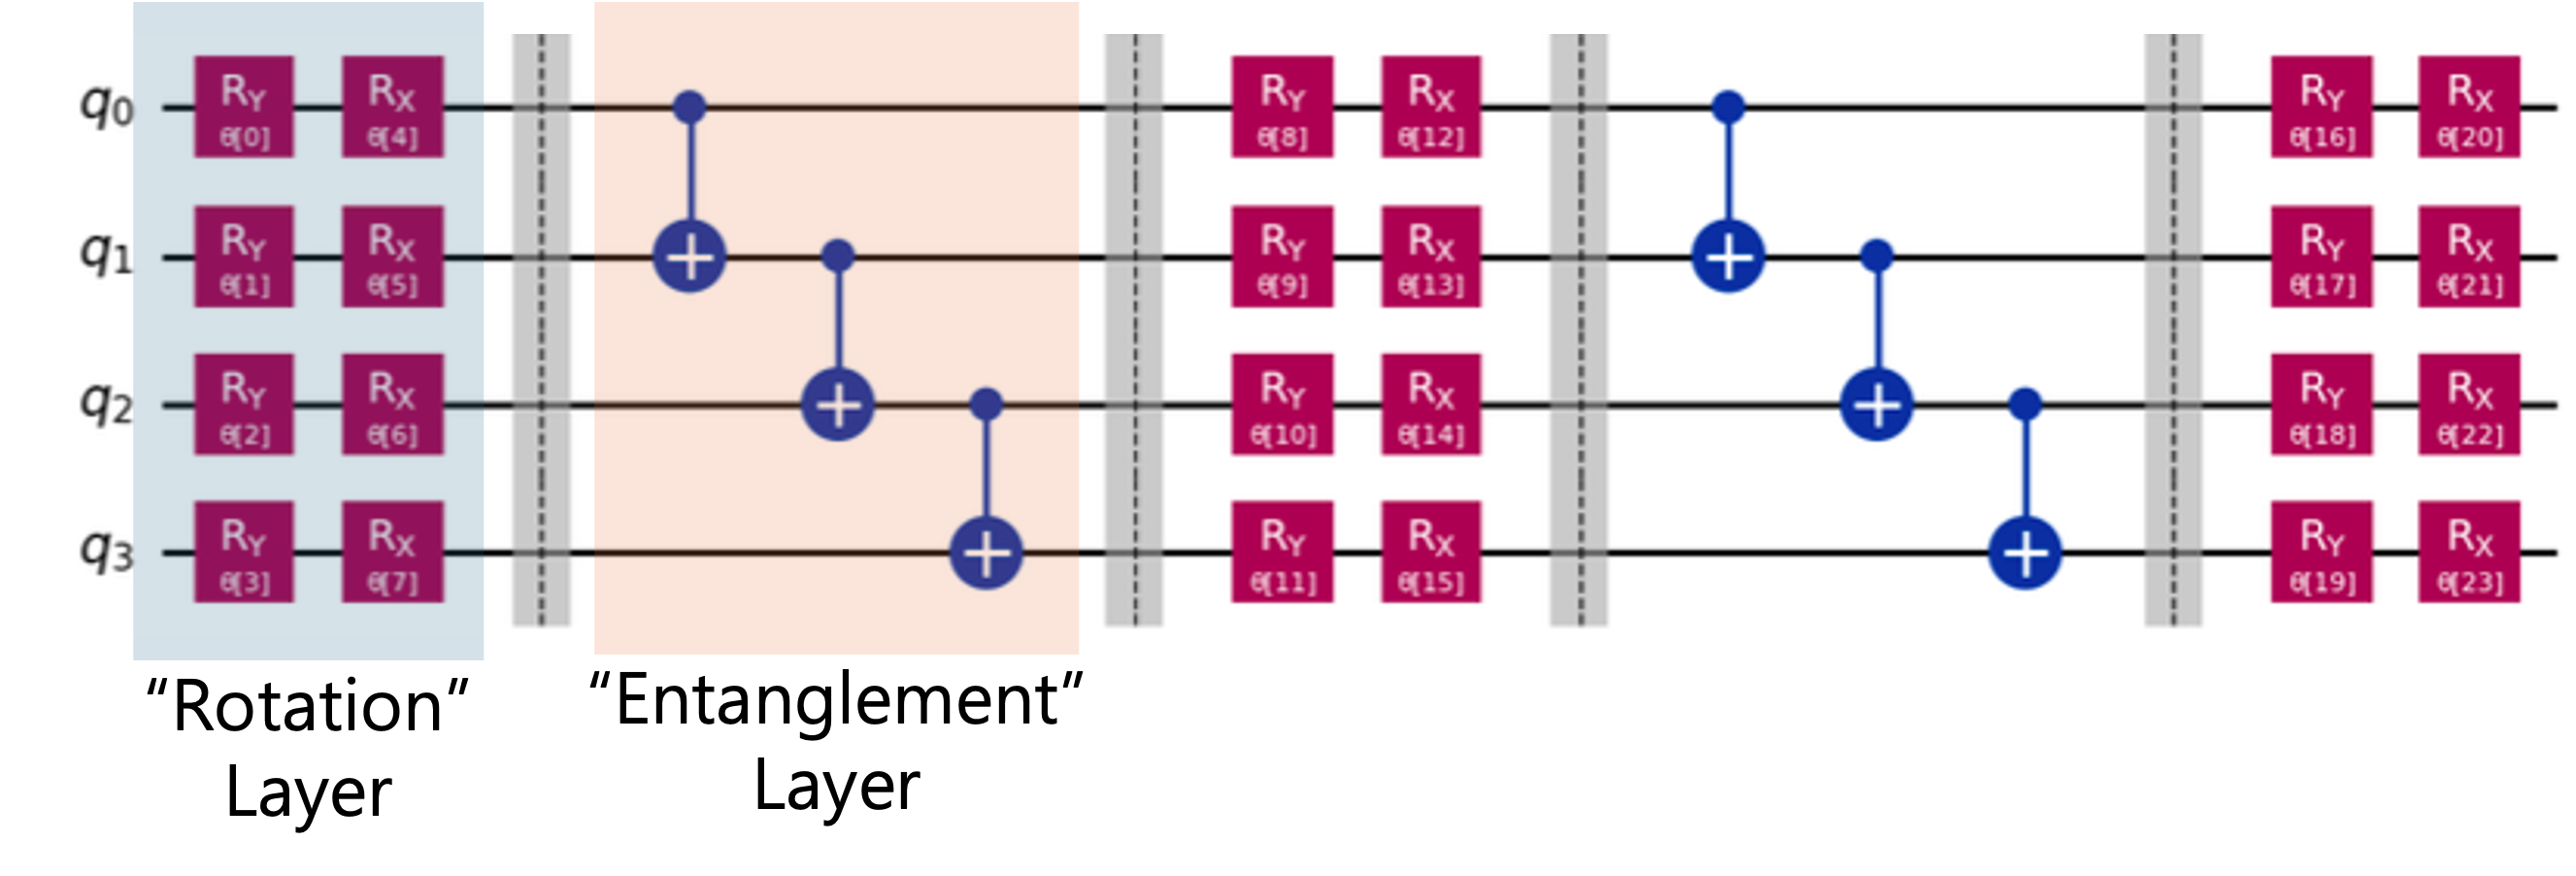
\includegraphics[width=0.8\textwidth]{fig/twolocal.png}
  \caption{twolocal Circuit}
  \label{fig:example3}
\end{figure}

임의의 single qubit의 양자상태는 두개의 Rotation Gate를 통해 만들 수 있다는점에 착안하여, 
두개의 Rotation Gate로 이루어진 Rotation Layer 와 Multi qubits 시스템이 갖는 특징인 Entanglement 를 CNOT 게이트로 구성된 Entanglement Layer를 번갈아여 구성하여
임의의 양자상태를 Rotation Gate의 각도를 파라미터로하여 표현하도록 하는 Ansatz이다. 이러한 Ansatz를 twolocal 혹은 Efficient SU2 라고 한다. 

둘째로는 문제에 조금더 특화된 Ansatz가 있을것이다. 기존의 양자화학계산인 FCI 에서의 계산방법에 착안하여
분자가 가질 수 있는 여러 Configuration들에 대응되는 Slater Determinant 를 basis로 양자상태를 표현한다. 
이때 각 Configuration은 어떤 기준상태로부터의 Excitation으로 기술 될 수 있으며, 따라서 각 Configuration은 생성/소멸 연산자로 표현될 수 있다. 
이렇게 문제에 맞는 헤밀토니안을 구성하고, 이를 파울리 게이트로써 Mapping 하게되면, 헤밀토니안에 잘 맞는 Ansatz를 구성할 수있으며, 이러한 형태의 Ansatz를 UCCSD Ansatz라고 한다. 
\end{enumerate}

\begin{enumerate}[label=\(\mathrm{iii}\))]
\item {에너지 계산}

우리가 계산해야할 것은, \(\langle \psi|H|\psi \rangle\) 이고, \(\mathrm{ii}, \mathrm{iii}\) 과정을 통해 임의의 파라미터화 된 양자상태(Ansatz)와 헤밀토니안을 구성하였다. 
우리가 가진 헤밀토니안의 형태는 \(\hat{H} = \sum_{a} \omega_a P_a\) 와 같고, 따라서 식을 아래와같이 정리 할 수있다. 
\begin{align*}
\langle \psi|H|\psi \rangle &= \langle \psi|\sum_{a} \omega_a P_a|\psi \rangle \\
&=\sum_{a} \omega_a \langle \psi|P_a|\psi \rangle
\end{align*}
여기서 하나의 \(P_a\) 에 대해서는 양자회로의 Projective Measurement 를 통해 그 기댓값을 계산하는것이 가능하다. 
따라서, Classical Optimizer를 통해서 계산된 값이 작아지도록 최적화 하면, 그 계산된 에너지가 VQE를 통해 계산된 에너지가 되고, 그 결과가 바닥상태에너지와 가까울 것이다.
\[
E_{VQE} =\min_\theta E(\theta) = \min_\theta \sum_{a} \omega_a \langle \psi(\theta)|P_a|\psi(\theta)\rangle
\]

\end{enumerate}
이런식으로 계산이 되는것이 VQE 알고리즘이다. 정말로 기존의 Variational Method 에서 기댓값 계산(에너지 계산) 부분만 양자컴퓨터로 바꿔치기 한 이야기 이다. 
이때, 각 양자컴퓨터에서 필요한 큐비트 수는 시스템의 스핀오비탈수와 같고, 따라서 QPE에 비해 필요한 큐비트가 적어 지금의 NISQ 시대에서도 효과적으로 사용할 수 있을것이라고 기대받고있고 많은 연구가 이루어지고있다. 
하지만 현재 이 방식에도 보완할 점이 있다. 우선, 에너지의 계산이 최적화과정에 의존한다는점이다. 최적화가 제대로 되지 않으면(실제로 제대로 잘 되지 않는다.) 에너지가 실제 이론값과 많은 차이를 보인다. 그리고, 위의 계산과정에서 보이는것처럼,
파울리스트링의 개수만큼 회로의 측정이 필요하다. 이는 시스템이 커질때마다 크게 증가하게된다. 

% Please add the following required packages to your document preamble:
% 
\begin{center}
\begin{tabular}{@{}ccccccc@{}}
\toprule
                   & \(H_2\) & LiH & \(H_2O\) & Co-O(single) & Co=O(Double) & LiCoO2((6,6),12)          \\ \midrule
\# of Pauli string & 15   & 631 & 1086  & 1545         & 2869         & \multicolumn{1}{c}{15017} \\ \bottomrule
\end{tabular}
\end{center}

이러한 특성들은 VQE를 실제 분자들에 적용하기 힘들게 만들기 때문에, 이를 해결하기위한 방법들이 연구가 되고있다. 지금부터 소개할 HI-VQE도 마찬가지로 이를 해결하기 위한 방법으로써 제시되었다.
\end{enumerate}
\newpage

\section{Method}
HIVQE는 양자화학 계산중 하나인 SCI로 부터 아이디어를 얻은 알고리즘이며, 이 SCI는 FCI의 단점을 보완하기위해 제안된 알고리즘이다. 
따라서 HIVQE를 이해하기 위해서는 FCI등, 기존의 양자화학 계산은 어떻게 진행되는지 이해해야 수월할것이다. 따라서 그러한 내용을 먼저 다뤄보자. 

\subsection{How to Express \(|\psi \rangle\) ?}
FCI던 VQE 던 뭐든 계산하고자 하는것은 \(\langle \psi|H|\psi \rangle\) 이다. 이것을 얼마나 정확히,
그리고 효율적으로 계산할 수있는가가 여러 알고리즘들의 목적이 될것이다. 그리고 여기서 hamiltonian \(H\) 는 이미 알려져 있으니, 계산을 위해서는 우리가 보고자 하는 분자의 파동함수를 어떻게 기술하는지 알아야할것이다.
우리는 양자역학에서 배웠듯이, "원자" 에 대해서는 \(n,l,m\) 등의 양자수들로 표현되는 오비탈들의 결합으로 표현된다는것을 알고있다.
이러한 오비탈의 경우는 이해가 되온바가 있기때문에, 원자에 대해서는 파동함수를 표현할 수 있다. 하지만 분자의 경우는 그렇지 않다. 
여러 원자가 모여 분자를 형성하며 각 원자들의 오비탈이 섞여서 원자와는 다른 구조를 이루게 되고, 따라서 이는 우리가 이해하기 힘들다. 
그래서 분자의 파동함수를 어떻게 표현할것인가? 에 대한 논의를 이 섹션에서 정리해볼것이다.
이 논리의 흐름은 N차원 공간 \(S\)에서 N개의 직교벡터 \(\left\{b_i\right\}\)를 찾으면, 그 벡터집합\(\left\{b_i\right\}\)은 공간 \(S\)의 직교 basis가 됨을 이용해서, 
분자 파동함수가 있을 공간을 잘 정의하고, basis를 잘 찾는 과정이 될것이다. 

\subsubsection{Fermionic System}
우리는 지금 분자를 다루고 있고, hamiltonian의 형태를 보면 알 수있듯이, 전자의 좌표,성질 등에 의존하는 시스템을 다루고있다. 이 전자들은 어떤 대칭성을 갖고있으며, 이 대칭성은 우리가 파동함수를 다루는데에 있어서 중요한 열쇠가 될것이다. 

전자는, Identical particle이다. 그리고, 이러한 Identical한 입자가 갖는 성질은 이름 그대로 모든 입자들이 모두 똑같아서 구별 불가능(indistinguishable)하다는 것이다. 
그렇다는것은, 두개의 Identical한 입자가 있을때, 그 두개의 입자의 위치를 맞바꾸더라도, 우리가 보는 현상은 똑같아야 한다는것이다. 
이를 조금더 수식적으로 이해해보자. i,j 번째 입자의 위치를 맞바꾸는 연산자인 \(\mathbb{P}_{ij}\) 연산자를 생각해보며 아래의 시스템을 보자. 

\begin{figure}[htbp]
  \centering
  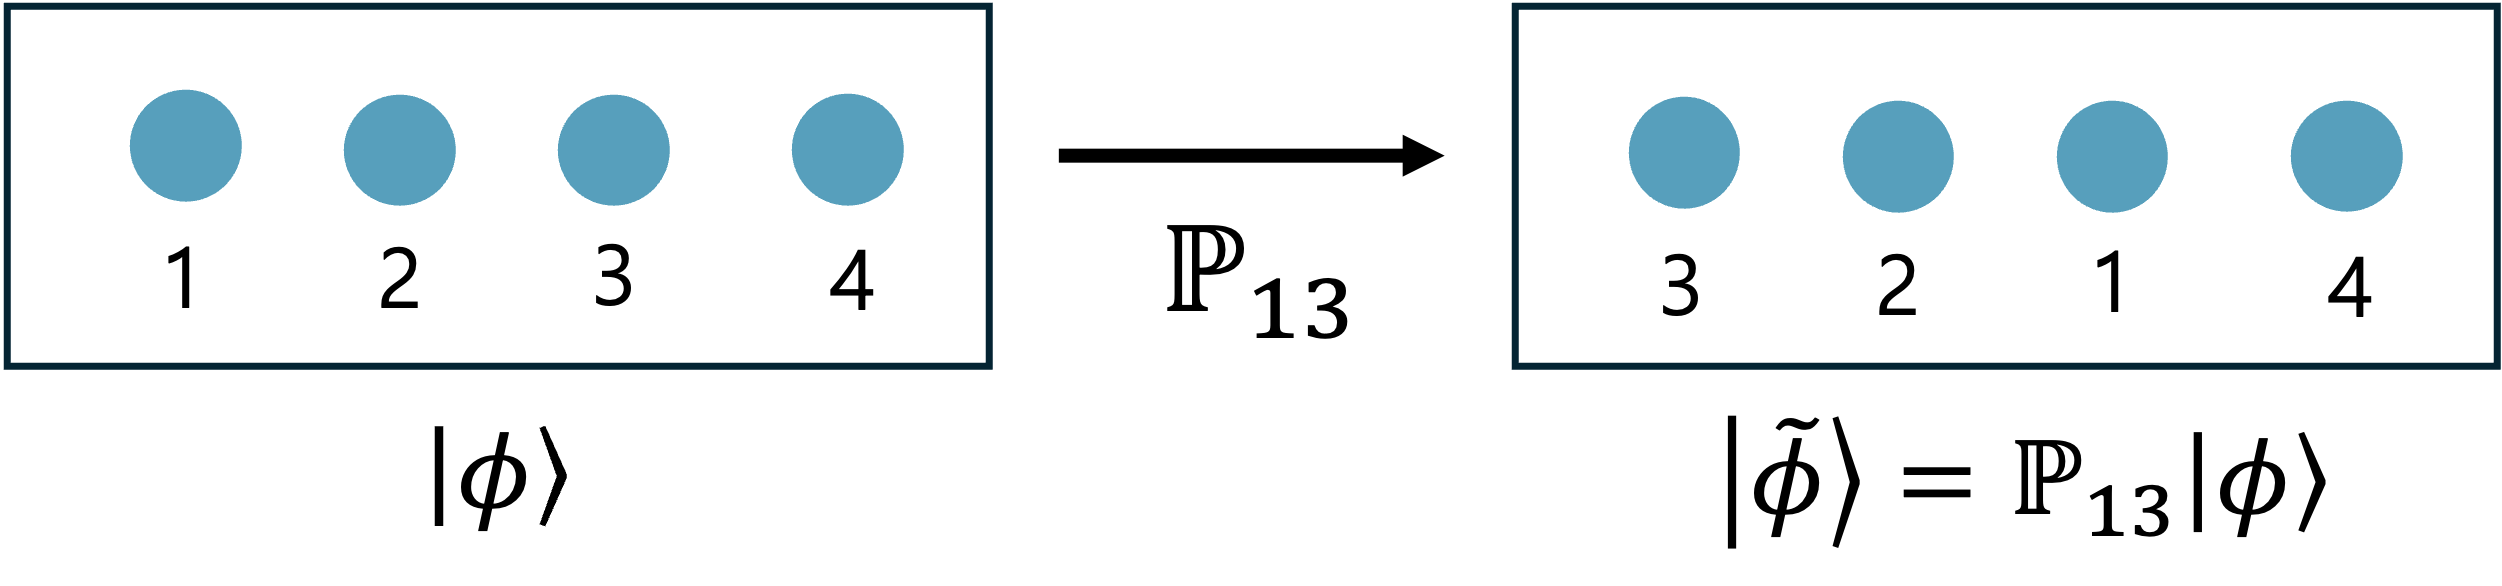
\includegraphics[width=0.8\textwidth]{fig/ident.png}
  \caption{System of Identical Particles}
  \label{fig:example2}
\end{figure}
\(\vert \tilde{\phi} \rangle\) 와 \(\vert \phi \rangle\)는 Identical particle 이므로 물리적으로 같은 현상을 기술해야한다. 즉, 같은 확률분포를 가져야한다. 따라서 아래와같이 쓸 수 있다. 
\begin{align*}
\mathbb{P}_{ij}\vert \phi \rangle &= \vert \tilde{\phi} \rangle \\
&= \lambda \vert \phi \rangle,\quad (\lambda \in \mathbb{C})
\end{align*}
즉, \(\lambda\)는 \(\vert \phi \rangle\)의 basis 에서 \(\mathbb{P}_{ij}\)  의 고유값이 된다. 

여기서 \(\vert \tilde{\phi} \rangle\)에 대해서 같은 인덱스의 \(\mathbb{P}_{ij}\) 연산자를 가한다면, Identical particle의 정의에 의해 \(\vert \phi \rangle\)와 같아야한다. 
\[
\mathbb{P}_{13} \vert \tilde{\phi} \rangle = \vert \phi \rangle
\]
즉, 아래와같이 정리할 수 있고, 
\[
{\mathbb{P}_{13}}^2 \vert \phi \rangle = \vert \phi \rangle
\]
여기에 위의 \(\mathbb{P}_{ij}\)의 고유값에 대한 표현을 대입하면 아래와같이 정리할 수있다. 
\[
{\lambda}^2 \vert \phi \rangle = \vert \phi \rangle
\]
\[
\longrightarrow {\lambda}^2 = 1
\]
\[
\longrightarrow \lambda = \pm 1
\]

정리해보면, Identical particle로 이루어진 시스템에 대해서 두 입자의 위치를 서로 교환하는것은 실제 물리적인 현상은 완전히 같지만, 그 파동함수의 위상은 달라질 수 있고, 
그때의 위상이 +1인 경우와 -1인 경우가 있다. 
이때 이 위상이 +1 인 입자를 Boson 이라고하고, -1인 입자를 Fermion 이라고 한다. 

\begin{figure}[htbp]
  \centering
  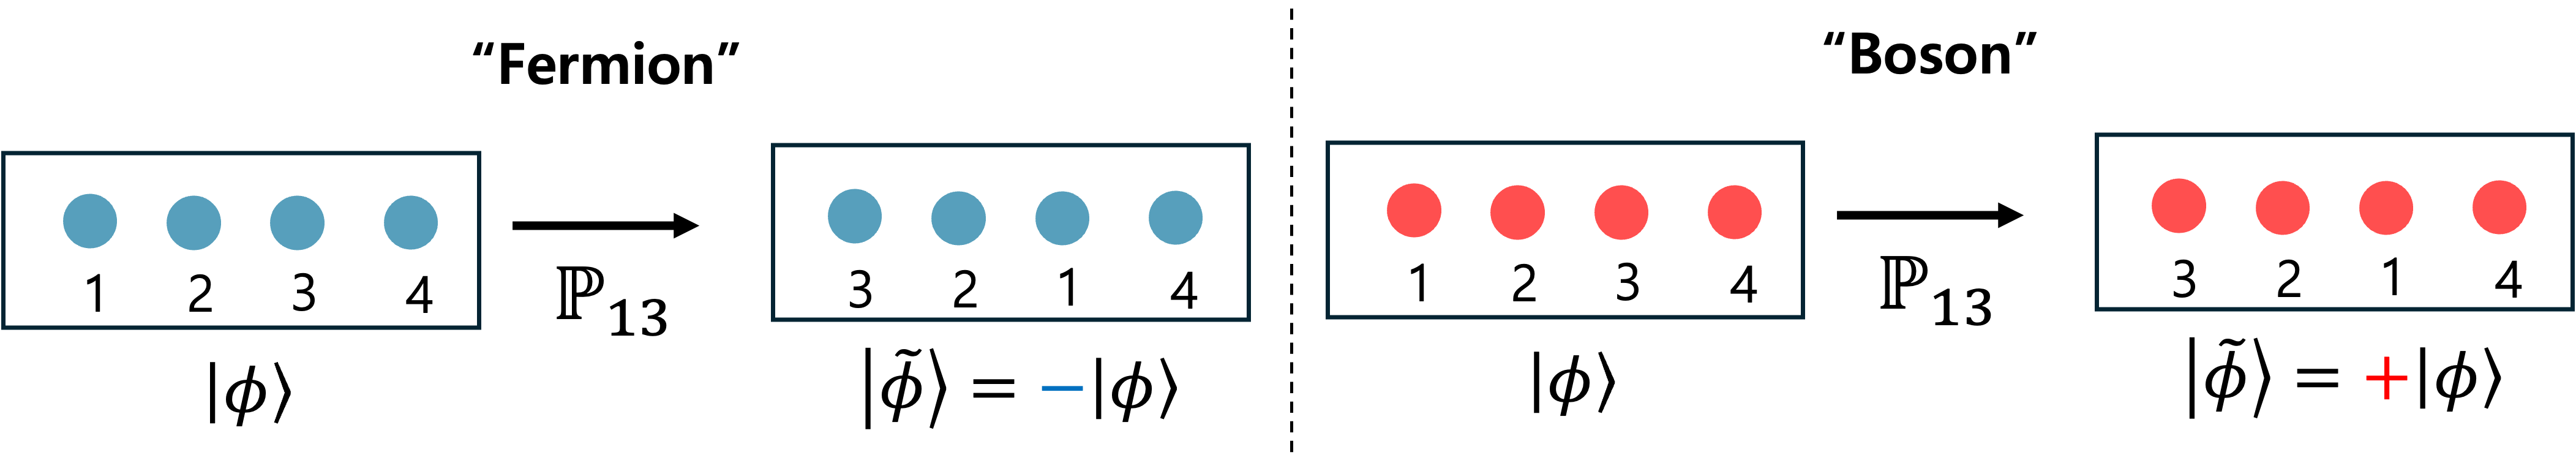
\includegraphics[width=0.9\textwidth]{fig/idet3.png}
  \caption{Bosons and Fermions}
  \label{fig:example2}
\end{figure}

우리가 다루는 시스템은 전자로 이루어져 있다고했고, 전자는 대표적인 Fermion 이다. 
즉, 우리가 구성해야할 파동함수는 전자에대한 정보(위치,스핀,...)들로 기술이 될텐데, 여기서 두 입자의 index를 바꾸는것에 대해서 시스템은 반대칭성을 가져야 한다는것을 알 수 있다. 
\[
\Psi_{fermion}(\dots, r_i, \dots, r_j, \dots) = -\Psi_{fermion}(\dots, r_j, \dots, r_i, \dots)
\]

\subsubsection{Slater Determinant}
이제 우리가 다룰것은 구체적으로 분자의 파동함수를 기술하고자 하는것이다. 그래서 어떤 형태일지 좀 구성을 해보자.
N-전자 파동함수에 대해서는 아래와같이 쓸 수 있다. 
\[
\Psi = \Psi(r_1, \dots, r_i, \dots, r_N)
\]
아러한 다변수함수를 다룰때, 물리학자들이 많이 하는접근은 모든 변수가 서로 독립인 상황을 보는것이다. 
물리적인상황으로는 각 전자들의 상호작용을 무시한다면, 아래와같이 적을 수 있다. (이러한 꼴로 표현하는것을  Product 라고한다.)
\[
\Psi(r_1, \dots, r_i, \dots, r_N)=\phi_1(r_1)\phi_2(r_2)\dots\phi_N(r_N)
\]
그런데 이러한 표현은 임의의 \(\phi_i\) 에 대해 입자들에 교환에 대해서 대칭이나 반대칭성을 부여하지 않는다. 
따라서 이러한 형태는 Identical particle 시스템을 다루기에는 적합하지 않다. 
임의의 \(\phi_i\) 에 대해서도 대칭성을 부여하기 위해서는 아래와같이 표현할 수 있다.
\begin{enumerate}[label=\(\mathrm{i}\))]
\item {\(N=2\)}
\[
\Psi(r_1,r_2)=\frac{1}{\sqrt{2}}[\phi_1(r_1)\phi_2(r_2)+\phi_1(r_2)\phi_2(r_1)],\quad (\text{bosonic System})
\]
\[
\Psi(r_1,r_2)=\frac{1}{\sqrt{2}}[\phi_1(r_1)\phi_2(r_2)-\phi_1(r_2)\phi_2(r_1)],\quad (\text{Fermionic System})
\]
\end{enumerate}
\begin{enumerate}[label=\(\mathrm{ii}\))]
\item {\(N=3\)}
\begin{align*}
\Psi(r_1,r_2,r_3)=\frac{1}{\sqrt{6}}&[\phi_1(r_1)\phi_2(r_2)\phi_3(r_3)+\phi_1(r_1)\phi_2(r_3)\phi_3(r_2) \\
&+\phi_1(r_2)\phi_2(r_1)\phi_3(r_3)+\phi_1(r_2)\phi_2(r_3)\phi_3(r_1)\\
&+\phi_1(r_3)\phi_2(r_1)\phi_3(r_2)+\phi_1(r_3)\phi_2(r_2)\phi_3(r_1)]\quad (\text{bosonic System})
\end{align*}
\begin{align*}
\Psi(r_1,r_2,r_3)=\frac{1}{\sqrt{6}}&[\phi_1(r_1)\phi_2(r_2)\phi_3(r_3)-\phi_1(r_1)\phi_2(r_3)\phi_3(r_2) \\
&-\phi_1(r_2)\phi_2(r_1)\phi_3(r_3)+\phi_1(r_2)\phi_2(r_3)\phi_3(r_1)\\
&+\phi_1(r_3)\phi_2(r_1)\phi_3(r_2)-\phi_1(r_3)\phi_2(r_2)\phi_3(r_1)]\quad (\text{Fermionic System})
\end{align*}
\end{enumerate}
우리가 볼것은 Fermionic System 이지만, 저 특성을 확인하기 위해 bosonic System도 같이 적었다. 
Fermionic System 의 파동함수에는 저렇게 -부호가 생기고, 이는 두 입자의 교환에 의해 생기는 위상이며, 이는 r에 붙어있는 인덱스들의 순열/역순열의 부호와 같다. 
반대로 Boson 에서는 입자교환에서 위상이 생기지 않기때문에, 모든 부호가 + 이다.
이러한 표현에서 N개 전자(Fermion)에 대한 임의의 표현을 적어보면 아래와같다. 

\[
\Psi(\mathbf{r}_1, \dots, \mathbf{r}_N) 
= \frac{1}{\sqrt{N!}} \det \begin{pmatrix}
\phi_1(\mathbf{r}_1) & \phi_2(\mathbf{r}_1) & \cdots & \phi_N(\mathbf{r}_1) \\
\phi_1(\mathbf{r}_2) & \phi_2(\mathbf{r}_2) & \cdots & \phi_N(\mathbf{r}_2) \\
\vdots & \vdots & \ddots & \vdots \\
\phi_1(\mathbf{r}_N) & \phi_2(\mathbf{r}_N) & \cdots & \phi_N(\mathbf{r}_N)
\end{pmatrix}
\]
\begin{center}
(Cf. Boson 에서는 Det 대신 perm 를 통해 기술할 수 있다.)
\end{center}

이렇게 행렬식의 꼴로 적으면, 시스템이 갖는 대칭성을 잘 부여할 수 있다는것을 이해했다. 이러한 꼴이 이제 Slater Determinant 로 이어질것이다. 
Slater Determinant 를 구성하기 위해서는 지금까지는 임의의 함수로 부여한 저 \(\phi\) 라는 친구가 어떤 꼴인지를 잘 정의하면 된다. 
\(\phi_i\) 라는 의미는 지금까지 \(i\) 번째 전자를 기술하기 위한 함수였다. 즉, \(i\) 번째 전자가 어떤 확률분포를 갖는지에 대한 정보, 즉 \(i\) 번째 전자의 파동함수에 대한 정보가 포함되어있어야한다. 
이러한 맥락에서 우리가 다루는 시스템은 지금까지는 "원자" 이고, 그 원자에서 어떤 전자들이 특정한 확률분포를 가지는것을 기술하기에 논리적으로 합당한것은 바로 "오비탈"이다. 
그래서 지금부터는 저 둘의 인덱스를 따로 부여하자. 
\[\phi_a(r_i)\]
이제부터는 이렇게 쓰고,이는 i번째 전자가 a오비탈을 점유한 상황을 나타낸다. 이거를 기반으로 아까 그 행렬식꼴을 다시쓴다면 아래와같다. 
\[
\Psi(\mathbf{r}_1, \dots, \mathbf{r}_N) 
= \frac{1}{\sqrt{N!}} \det \begin{pmatrix}
\phi_a(\mathbf{r}_1) & \phi_b(\mathbf{r}_1) & \cdots & \phi_M(\mathbf{r}_1) \\
\phi_a(\mathbf{r}_2) & \phi_b(\mathbf{r}_2) & \cdots & \phi_M(\mathbf{r}_2) \\
\vdots & \vdots & \ddots & \vdots \\
\phi_a(\mathbf{r}_N) & \phi_b(\mathbf{r}_N) & \cdots & \phi_M(\mathbf{r}_N)
\end{pmatrix}
\]
여기서, a,b,c 는 반드시 연속이지 않아도 된다. 
이거에대한 이야기는 조금더 뒤에 다루겠지만, M개의 오비탈이 있고, N개의 전자가 있다고할때, 일반적으로 M이 N보다 크다. 
그래서 그 오비탈들에게 1,2,3 이렇게 index 를 준다고 했을때, 분명 전자가 점유되지 않은 오비탈도 존재하게되고, 그 빈 오비탈은 고려되지 않기때문이다. 

이제 마지막 논리 이다. 그럼 저 오비탈이라고 한 \(\phi\)가 우리가 흔히 아는 1s, 2s, 2p 뭐 그런 오비탈들이냐? 하면 반은 맞고 반은 틀리다.
그렇게 파동함수를 기술하게되면, 예를들어 전자가 두개인 시스템을 다시 돌아가보자. 
\[
\Psi = \Psi(r_1,r_2)
\]

라고했는데, 
여기서 \(r_i\)라고하는것은 엄밀하게는 스핀까지 포함해야한다. 따라서 아래와같이 쓸 수 있다. 
\begin{align*}
r_i &= x_i s_i\\
x_i &: \text{Spartial coordinate of i-th Electron}\\
s_i &: \text{Spin coordinate of i-th Electron} \in \left\{-\frac{1}{2}, \frac{1}{2}\right\}
\end{align*}

따라서 
\begin{align*}
\Psi(r_1,r_2)&=\Psi(x_1,s_1, x_2,s_2)\\
&=\psi(x_1, x_2)\chi(s_1,s_2)
\end{align*}
와 같이 써지게 되고, 앞선 행렬식에서 \(\phi\)를 흔히 아는 오비탈로 택하면,이는 공간 Part 만을 다루는것이므로, 아래와같이 기술된다. 
\[
\Psi(x_1,s_1, x_2,s_2) = \frac{1}{\sqrt{2}}[\phi_1(r_1)\phi_2(r_2)-\phi_1(r_2)\phi_2(r_1)]\chi(s_1,s_2)
\]

이때, \(\frac{1}{\sqrt{2}}[\phi_1(r_1)\phi_2(r_2)-\phi_1(r_2)\phi_2(r_1)]\) 파트는 앞서 정의하기를 언제 Anti-Symmetry 하도록 구성을 하였다. 
따라서 전체 파동함수가 Anti-Symmetry 이려면 \(\chi(s_1,s_2)\) 이 파트는 Symmetry 여야만 한다. 
하지만, \(\chi(s_1,s_2)\)는 두개의 스핀의 덧셈이므로, 두전자의 스핀좌표가 같다면 스핀의 덧셈규칙에 의해 Singlet 상태또한 하나의 스핀상태가 되게 된다. 
여기서 Singlet 상태는 두 스핀의 교환에 대해서 Anti-Symmetry 하므로, 이경우에는 전체 파동함수(공간 + 스핀)이 입자의 교환에 대해 대칭인 함수가 된다. 
따라서, 이렇게 기술하는것은, 올바르게 시스템의 반대칭성을 기술할 수 없게된다. 
그래서 \(\phi\)는 아래와같이 Spartial-part 와 Spin-part 를 모두 기술하는 소위 스핀오비탈로써 택하게 된다. 
\[
\phi_a(r_i) = \psi(x_i)\chi(s_i)
\]

이렇게 기술하게되면, 
행렬식으로 표현된 파동함수가 전체 시스템을 기술하는 파동함수가 되어, spin과는 상관 없이 시스템의 반대칭성을 만족할 수 있다. 

이렇게 각 전자의 spin-orbital 파동함수를 이용하여, Anti-Symmetry를 만족하기 위해 행렬식의 꼴로 전체 시스템의 파동함수를 적은 꼴을 \enquote{\textbf{Slater Determinant}} 라고 한다. 
이 Determinant가 시스템이 만족해야할 성질들을 만족하는지 Check 해보자. 
\[
\Psi(\mathbf{r}_1, \dots, \mathbf{r}_N) 
= \frac{1}{\sqrt{N!}} \det \begin{pmatrix}
\phi_a(\mathbf{r}_1) & \phi_b(\mathbf{r}_1) & \cdots & \phi_M(\mathbf{r}_1) \\
\phi_a(\mathbf{r}_2) & \phi_b(\mathbf{r}_2) & \cdots & \phi_M(\mathbf{r}_2) \\
\vdots & \vdots & \ddots & \vdots \\
\phi_a(\mathbf{r}_N) & \phi_b(\mathbf{r}_N) & \cdots & \phi_M(\mathbf{r}_N)
\end{pmatrix}
\]


\begin{enumerate}[label=\(\mathrm{i}\))]
\item {Anti-Symmetry}

두 입자의 교환은 행렬식의 관점에서 r의 인덱스를 서로 맞바꾸는 것이고, 이는 행렬식에서 두개의 행을 바꾸는것과 같다.
그리고, 선형대수의 지식을 써먹어보면, 행렬식에서 두 행을 맞바꾸는것은 전체 행렬식에 - 부호를 붙히게 된다. 
\end{enumerate}

\begin{enumerate}[label=\(\mathrm{ii}\))]
\item {Pauli exclusive Principle}

파울리의 배타원리는, 한 오비탈에 같은 스핀전자가 두개 점유하는 경우는 물리적으로 옳지 않다 라는 내용이다. 
이거를 우리의 상황에 맞게 조금 언어를 바꿔보면, 한 스핀오비탈을 두개의 전자가 점유하는것은 물리적으로 옳지 않다. 라고 해석하면 된다. 
한 스핀오비탈을 두개의 전자가 점유하는것? 이건 phi 에 달려있는 index가 같은열이 있다는 소리이다. 
그리고 마찬가지로 선형대수의 지식을 끌어오면, 두 열이 같으면, 행렬식은 0이된다. 
즉, 파울리의 배타원리를 위배하도록 파동함수를 작성하면, 자동으로 파동함수는 0이된다. 
\end{enumerate}
이제 이러한 Slater Determinant를 일일히 적을 수 없으니 아래와같이 표현한다. 
\begin{align*}
\Psi(\mathbf{r}_1, \dots, \mathbf{r}_N) 
&= \frac{1}{\sqrt{N!}} \det \begin{pmatrix}
\phi_a(\mathbf{r}_1) & \phi_b(\mathbf{r}_1) & \cdots & \phi_M(\mathbf{r}_1) \\
\phi_a(\mathbf{r}_2) & \phi_b(\mathbf{r}_2) & \cdots & \phi_M(\mathbf{r}_2) \\
\vdots & \vdots & \ddots & \vdots \\
\phi_a(\mathbf{r}_N) & \phi_b(\mathbf{r}_N) & \cdots & \phi_M(\mathbf{r}_N) 
\end{pmatrix} \\
& \equiv \vert \phi_a \phi_b \dots \phi_M\rangle
\end{align*}
즉, 각 전자들이 점유한 오비탈을 통해 Determinant 를 표현할 수 있다. 



\subsubsection{Occupation number Representation}


Slater Determinant의 표현을 지금은 \enquote{어떤 전자가} 어떤 오비탈을 점유했는가를 통해 표현하고 있는데, 
사실 모든 전자는 Identical 하므로, 이를 \enquote{어떤 오비탈}이 전자가 점유 되었나 안되었나 만을 표기하면 될 것이라는 맥락에서 이렇게 표현을 바꿔보자는 것이다. 
이렇게 하면, 이전의 표현 \(\vert \phi_a \phi_b \dots \phi_M\rangle\)에서는 두 \(\phi\)를 바꾸는것이, 결국 전자 두개를 교환하는것 이므로, 상태 자체에서 Anti Symmetry를 갖게된다. 
하지만 미리 스포를 하자면, 이후의 설명에서는 모든 전자를 정말로 Identical 하게 보아, 상태에서는 전자의 교환이 정의 될 수 없고, 이러한 교환을 operator 로써 표현하여, 이 operator에 Anti Symmetry를 부여하여 시스템을 다루게 될것이다. 
이후 헤밀토니안도 이 basis에 맞춰 생성/소멸 연산자를 정의하여 헤밀토니안을 그 연산자를 통해 표현할것이다. 
이러한 과정을 Second Quantization 이라고 한다. 
\begin{figure}[H]
  \centering
  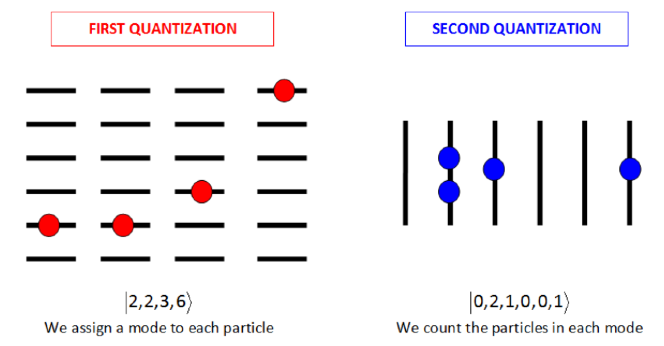
\includegraphics[width=0.7\textwidth]{fig/1to2.png}
  \caption{Second Quantization diagram}
  \label{fig:example2}
\end{figure}
그러기 위하여 아래와같이 number operator를 정의하자.
\[
\hat{n}_i : \text{number operator}
\]
여기서의 인덱스 \(i\)는 오비탈에 대응되는 인덱스 이다. 이 연산자의 형태는 이후 설명할것이고, 지금은 저 연산자의 역할을 이해해보자. 
이 연산자의 역할은 어떤 Slater Determinant 에 가해졌을때 i오비탈에 전자가 점유되었나 점유되지 않았나를 고윳값으로 반환한다. 즉, 아래와같이 표현된다. 
\[
\hat{n}_i | \Phi \rangle = n_i | \Phi \rangle, \quad n_i \in \{0,1\}
\]
이제 이 연산자를 왜 정의했냐 하면, 
지금의 \(\vert \phi_a \phi_b \dots \phi_M\rangle\) 이 표현은 
\[
= \vert \phi_a \phi_b \dots \phi_M \rangle \\
\hat{n}_i = \hat{a}_i^{\dagger}\hat{a}_i
\]





\subsubsection{Construct Molecular Wave Function}
자 이제 거의 다 왔다. 다시 우리가 하고자했던것을 되돌아보면 전체 시스템에 대해서 \(\langle \Psi|H|\Psi \rangle\)를 계산하고자 했던것이였고, 
여기서 \(|\Psi \rangle \)를 기술하기위해 지금까지 여러 논리들을 이어왔었다. 
잠시 Notation을 정리하고 가자. 
\begin{align*}
| \Psi \rangle &: \text{전체 시스템(분자)의 파동함수}\\
| \Phi \rangle &: \text{Slater Determinant}
\end{align*}
이제 분자의 시스템에 대해서 다뤄보자. 
간단하게 H2 의 시스템부터 가보자. 

\begin{figure}[htbp]
  \centering
  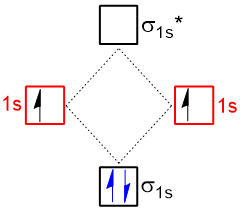
\includegraphics[width=0.4\textwidth]{fig/Moecular-Orbital-DiagramH2.png}
  \caption{H2 Molecular orbital diagram}
  \label{fig:example2}
\end{figure}

위의 그림이 잘 알려져있는 H2의 분자에서 오비탈이 어떤식으로 생성되는지를 보여주는 모식도 이다. 
빨간색으로 표시된것이 결합 전의 두개의 H 원자에 대한 오비탈의 모식도이다. 두 원자가 1s 오비탈을 각각 가지고 있을거고, 각 오비탈에는 전자 1개를 가지고 있다. 
그 두 원자가 결합하여 분자를 형성하며, 두개의 1s 오비탈은 파울리의 배타원리에 의해 같은 에너지를 가질 수 없으므로 Split 된다. 좀더 디테일하게는, 전자들의 스핀상태에 의해 에너지가 Split 되며, 
\(\sigma_{1s}\) 로 표시된 결합 오비탈이 Singlet 을 나타내며, \(\sigma_{1s}^*\) 로 표시된 반결합 오비탈이 Triplet 을 나타내게 된다. 그래서 반결합성 오비탈이 에너지가 더 높으므로, 그림에도 더 높게 그려져있다. 
이런식으로 가게될거라는건 정성적으로 이해하지만, 사실 \(\sigma_{1s}\) 의 함수의 형태가 어떤식인지는 알 수 없다. 
그래서 시스템의 파동함수를 \(\sigma_{1s},\sigma_{1s}^*\) 를 통해서는 기술 할 수 없고, 다른방식을 통해 기술해야하며, 그 방식이 바로 Slater Determinant를 이용하는것이다. 

가장 단순한 접근은 Slater Determinant 자체를 분자의 파동함수로써 사용하는것이다. 
하지만 하나의 시스템에서 Slater Determinant은 하나가 아니다. 
시스템이 M개의 스핀오비탈과 N개의 전자를 갖고있다면,  M개의 오비탈중 전자가 점유될 N개를 택하는 경우의수인 \(\binom{M}{N}\) 개의 Slater Determinant가 생기게 된다. 
여기서 M개의 오비탈중 N개의 전자가 점유된 하나의 그 상황을 Configuration이라고 하고, 그에 대응되는 Slater Determinant를 앞서 정의한대로 쓸 수 있다. 
여기서 각 Slater Determinant는 각 원자의 Spartial Part에 대응될 1s 오비탈의 파동함수와 Spin Part 에 대응될 \(Y^l_m\) 으로 그 형태를 적을 수 있고, 따라서 각 Determinant 에 대해 \(\langle \Phi_i|H|\Phi_i \rangle\) 를 계산 할 수 있다. 
모든 Slater Determinant 중, \(\langle \Phi_i|H|\Phi_i \rangle\) 값이 가장 작은 상태가 우리가 보고자 하는 바닥상태에 가장 가까운 상태일것이므로, 그 상태를 분자의 파동함수로 사용할 수도 있고, 
이러한 계산방법을 Hartree-Fock 계산 이라고 한다. 
하지만 이런 Hartree-Fock (HF) 계산은 정말 단순히 두개의 원자 오비탈만을 가지고 기술하는것이므로, 정확하지는 않다. 그래서 이러한 HF 계산보다 조금더 정밀한 계산을 필요로하고, 그러한 계산을 post-HF 계산이라고한다. 
이후 다루게될 모든 양자계산들은 이러한 Slater Determinant를 이용한 post-HF 계산이다. 
그래서 이러한 Slater Determinant를 가지고 전체 분자의 파동함수를 어떻게 기술할것인가? 가 관건인데, 여기에는 두가지 논리가 있다. 둘다 논리적으로 틀리지는 않지만, 두번째의 경우가 조금더 엄밀하다는 느낌이 있다. 

\begin{enumerate}[label=\(\mathrm{i}\))]
\item {Linear Algebra Ver.}

\end{enumerate}

\begin{enumerate}[label=\(\mathrm{ii}\))]
\item {Exterior Algebra Ver.}

\end{enumerate}



N개의 전자로 이루어진 시스템에 대해서, 각 전자의 정보 (위치,스핀,...)들의 좌표로 기술되는 함수로 구성되는 Hilbert Space \(\mathcal{H}_N\)이 있을것이고, 우리가 다루는 파동함수는 그러한 \(\mathcal{H}_N\) 에서 기술될것이다. 
그리고 \(\mathcal{H}_N\) 은 전자 한개에 대한 Hilbert space \(\mathcal{H}_1\) 의 N번의 텐서곱으로 표현될것이다. 
\[
\mathcal{H}_N = (\mathcal{H}_1)^{\otimes N}
\]
여기서,
\begin{align*}
\mathcal{H}_1 &=  L^2(\mathbb{R}^3 \times \{\uparrow, \downarrow\}) \\
L^2 (\left\{b\right\}) &: \left\{b\right\} \text{를 basis로 구성된 공간에서 제곱적분 가능한 함수의 공간} \\
\mathbb{R}^3 &: \text{전자 하나의 위치를 기술하기 위한 basis 집합}\\
\{\uparrow, \downarrow\} &: \text{전자 하나의 스핀을 기술하기 위한 basis 집합}
\end{align*}

그리고 이러한 \(L^2(\mathbb{R}^3 \times \{\uparrow, \downarrow\})\) 공간은 Spin orbital로 구성된 집합이 Span 한다 라는것이 알려져있다. 
(이부분 아직 모르곘음.,~Sturm–Liouville 정리..? )
무한하면 Complete하다 인데, 무한개가 있을 수 있나? Virtual 을 생각하는건가?? 
일단 넘어가자. 
아무튼 아래와 같이 정리 할 수 있고 
\[
\mathcal{H}_1^{(M)} := \text{span} \{ \varphi_1, \dots, \varphi_M \} \subset \mathcal{H}_1
\]
따라서 전체 시스템의 Hilbert space 는 아래와같이 쓸 수 있다 
\[
\mathcal{H}_N^{(M)} := \left( \mathcal{H}_1^{(M)} \right)^{\otimes N}
\]

하지만 이러한 표현은 Fermion의 Anti-Symmetry 가 고려되지 않은 공간이다. 이러한 Anti-Symmetry 를 만족하는 어떤 subspace \(\mathcal{H}_N^{anti}\)에 우리가 구성하고자 하는 파동함수가 있을것이다. 
\[
\vert \Psi \rangle \in \mathcal{H}_N^{anti} \subset \mathcal{H}_N
\]
이러한 \(\mathcal{H}_N^{anti}\)를 수학적으로 아래와같이 구성할 수 있다. 


\begin{align*}
\mathcal{H}_N^{\text{anti}} &= \bigwedge^N \mathcal{H}_1\\
&= \mathcal{H}_1 \wedge \mathcal{H}_1 \wedge \dots \wedge \mathcal{H}_1
\end{align*}

여기서, 
\[
\mathcal{A} := \frac{1}{N!} \sum_{\pi \in S_N} (-1)^{\text{sgn}(\pi)} \hat{P}_\pi
\]

\subsection{FCI}
FCI에 관한 이야기를 다뤄보자. 그중에 FCI 는 모든 계산방법중 \(\langle \psi|H|\psi \rangle\)를 가장  \enquote{정확히} 계산하기 위한 계산방법이다. 
이 계산방식은 다른 양자화학 계산들의 기준값이 된다. (그니까 FCI 와 비교했을때 이만큼의 차이가 난다. 이런식으로) 그러한 FCI의 계산방법에 대해 이해해보자. 
앞의 section을 통해, 분자의 파동함수는 다음과 같이 Slater Determinant를 basis로 표현할 수 있다는것을 이해했다. 
\[
|\Psi\rangle = \sum_I c_I |\Phi_I\rangle
\]


\subsection{SCI}

\subsection{HIVQE}

\end{document}
